The propeller was quickly identified as one of the key components of the vehicle. The first step in designing a propeller was to analyse its design requirements. Looking at Equation \ref{eq:e}, it was made clear that propeller efficiency needed maximising to achieve the greatest possible speeds. Therefore, adequate parameters to ensure this high efficiency had to be chosen. One of the better ways to achieve this is to build a model.

\subsection{Design process}

Several models exist for the theoretical analysis of propellers and fans in general. The two main ones are the disk actuator theory and blade element theory. Disk actuator theory was deemed too basic for this application as the aim was to generate and analyse various blade geometries. It is not possible with this model as it treats the fan as a disk through which a pressure change occurs. Therefore, blade element theory was chosen.

A Python script was written that could produce simple blade planforms using a finite number of cross-sections (typically around 10). The code integrated Xfoil to use accurate lift and drag coefficients of different aerofoils over various angles of attack. The script would maximise efficiency for each cross-section at a desired operating point of the vehicle and output pitch and chord length (based on desired thrust distribution) profiles along the blade. The propeller was then tested at varying wind and group speeds to determine its performance at different operating conditions as shown in Figure \ref{fig:jamesresults}, demonstrating a maximum efficiency of over 90\%. Issues with convergence and the inability to incorporate Reynold’s number limited the expected reliability of this code but made a good starting point.

\begin{figure}[!htbp]
    \centering
    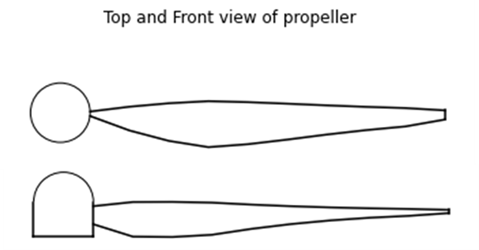
\includegraphics{images/part6/jamescode.png}
    \caption{Initial python script generated propeller profile}
    \label{fig:jamesprop}
\end{figure}
\begin{figure}[!htbp]
    \centering
    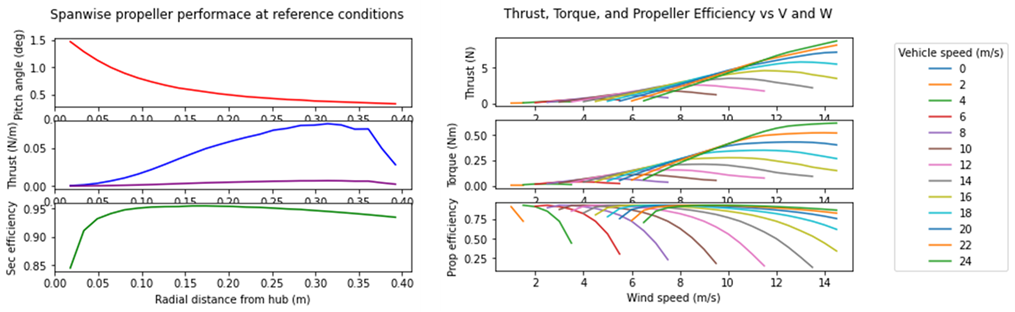
\includegraphics{images/part6/jamesresults.png}
    \caption{Performance of python-generated propeller blade at varying wind and ground speeds}
    \label{fig:jamesresults}
\end{figure}

In a second iteration, a new python script was written. The aim was to integrate JavaProp, a program that uses blade element theory. This code, developed by Martin Hepperle, had shown to produce satisfying results in generating blade geometries from inputs. It was also able to output their associated total force plot, and presented no issues with convergence. Testing demonstrated similarities between iterations 1 and 2 of the code, however, the latter was deemed more suitable due to the well-established reliability of JavaProp.

As shown in Figure \ref{fig:pyflowchart}, first, a set of parameters were defined for JavaProp to output the optimal propeller geometry for these conditions. Once the geometry was generated, it could then be tested by outputting the performance over the operational domain. Using the output, choosing the parameters was made easier. 

For the performance evaluation and to generate the plots shown in Figure \ref{fig:pythonresults}, it was required to integrate the equations defined in \cite{drela20dead}. The force of the wheels was obtained from the thrust generated by the propeller using Equation \ref{eq:fulleq}. Derivation for this equation is available in \cite{drela20dead}.

\begin{equation}
F_{n e t}=F_{p}\left\{1+\left[\frac{2 V \eta_{g} \eta_{v}}{(V-W)+\left((V-W)^{2}+\frac{2 F_{p}}{\rho A_{p}} \frac{1}{\eta_{\text{swirl }}}\right)^{\frac{1}{2}}}-1\right]^{-1}\right\}^{-1}
\label{eq:fulleq}
\end{equation}

Estimations were made for the different efficiency parameters. The overall propeller efficiency outputted by JavaProp was used for $\eta_p$ it was then used to compute the viscous efficiency $\eta_v$. For the swirl efficiency $\eta_{swirl}$, a conservative value of 0.95 was taken, as advised in \cite{drela20dead}. For the transmission efficiency $\eta_g$ a conservative value of 0.93 was taken after surveying common efficiency value ranges.

\begin{figure}[!htbp]
    \centering
    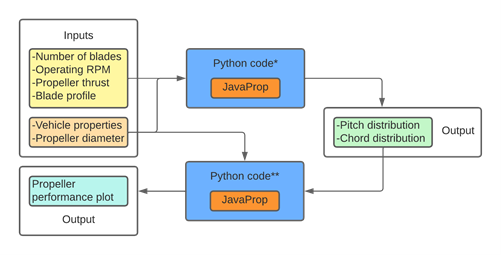
\includegraphics{images/part6/flowchart.png}
    \caption{DWFTTW theoretical model inputs and outputs. *Geometry generation from specific operating conditions. **Performance evaluation over various operating conditions}
    \label{fig:pyflowchart}
\end{figure}

Figure \ref{fig:pythonresults} shows how the performance of the propellers generated by JavaProp was evaluated. Force contours were plotted to study and better understand the various parameters of a propeller. It is important to note that blade element theory does not allow for zero inflow cases. This is the reason why the thrust estimated is 0 below the $\beta = 1$ line, as the relative wind is 0 or negative. The positive force zone outlines the domain in which the vehicle would theoretically be able to operate without the implication of any exterior forces.

\begin{figure}[!htbp]
    \centering
    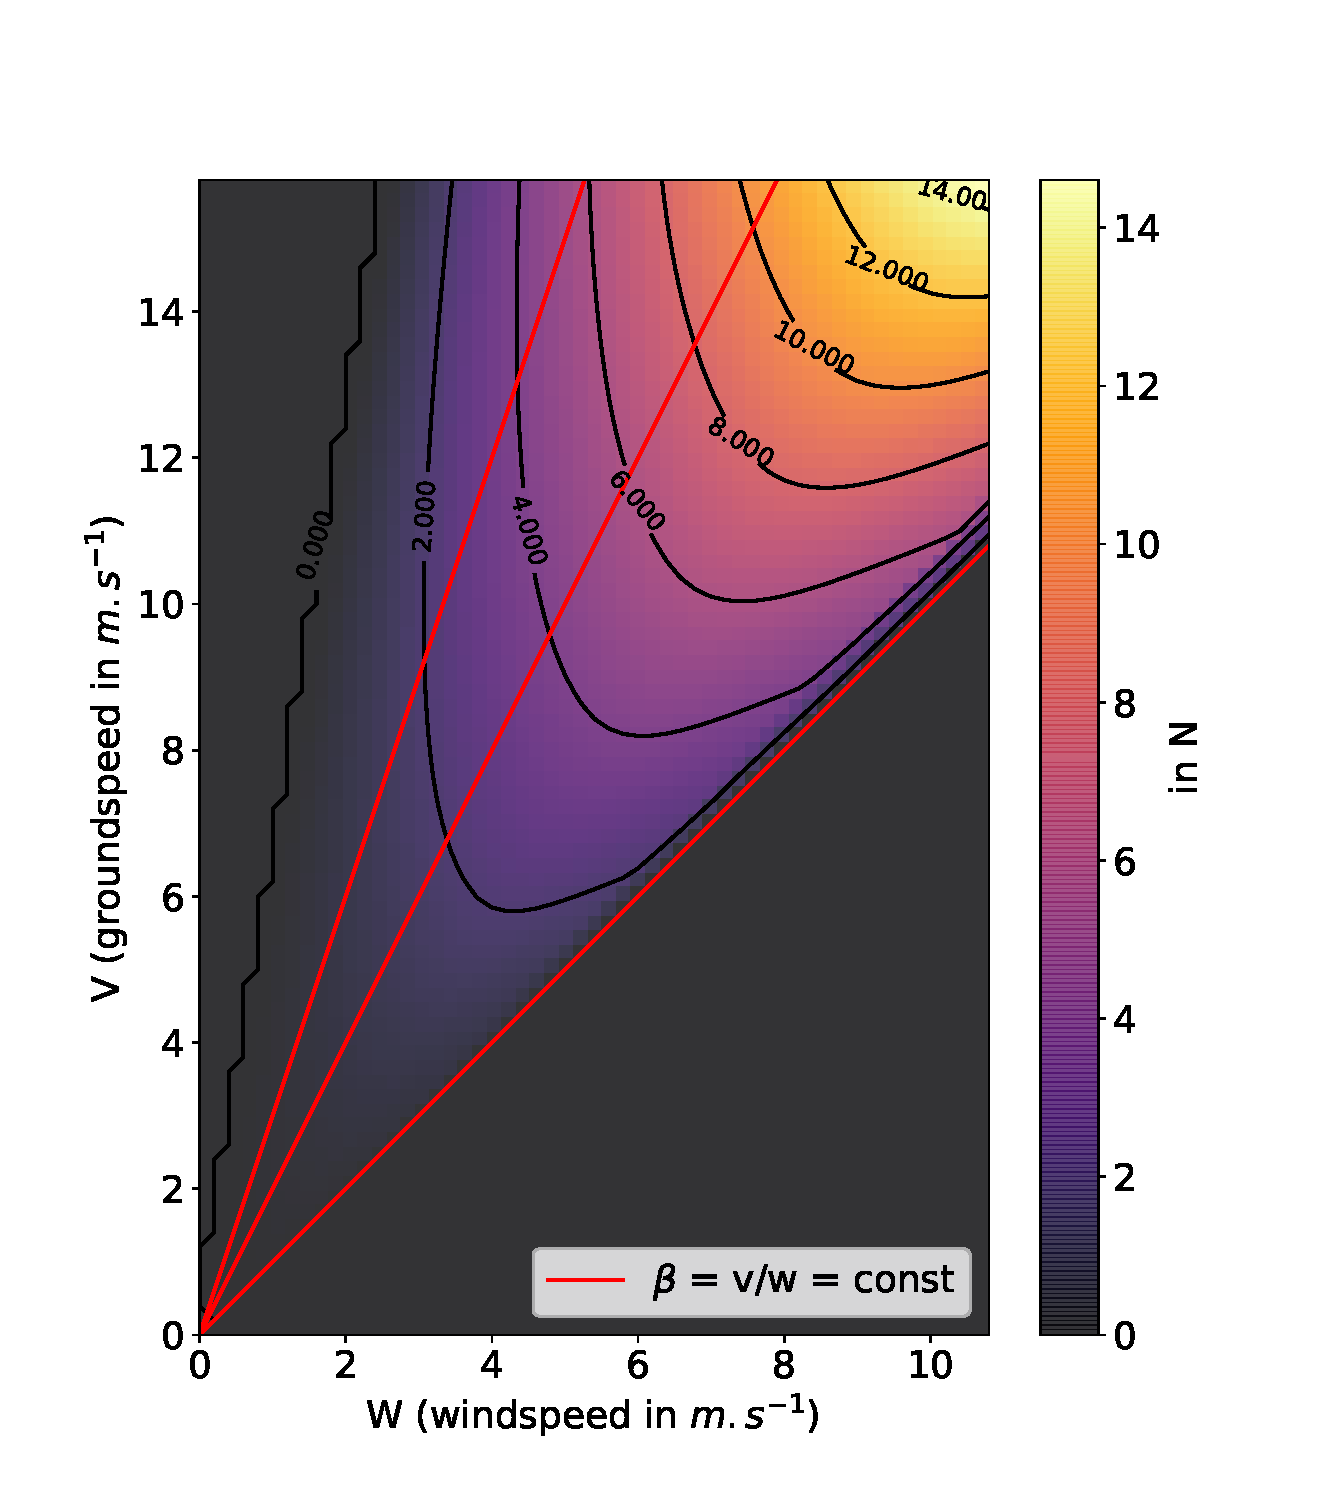
\includegraphics[width = 0.22\textwidth]{images/part6/naca6412-8a-78-10-5-3-470-6.pdf}
    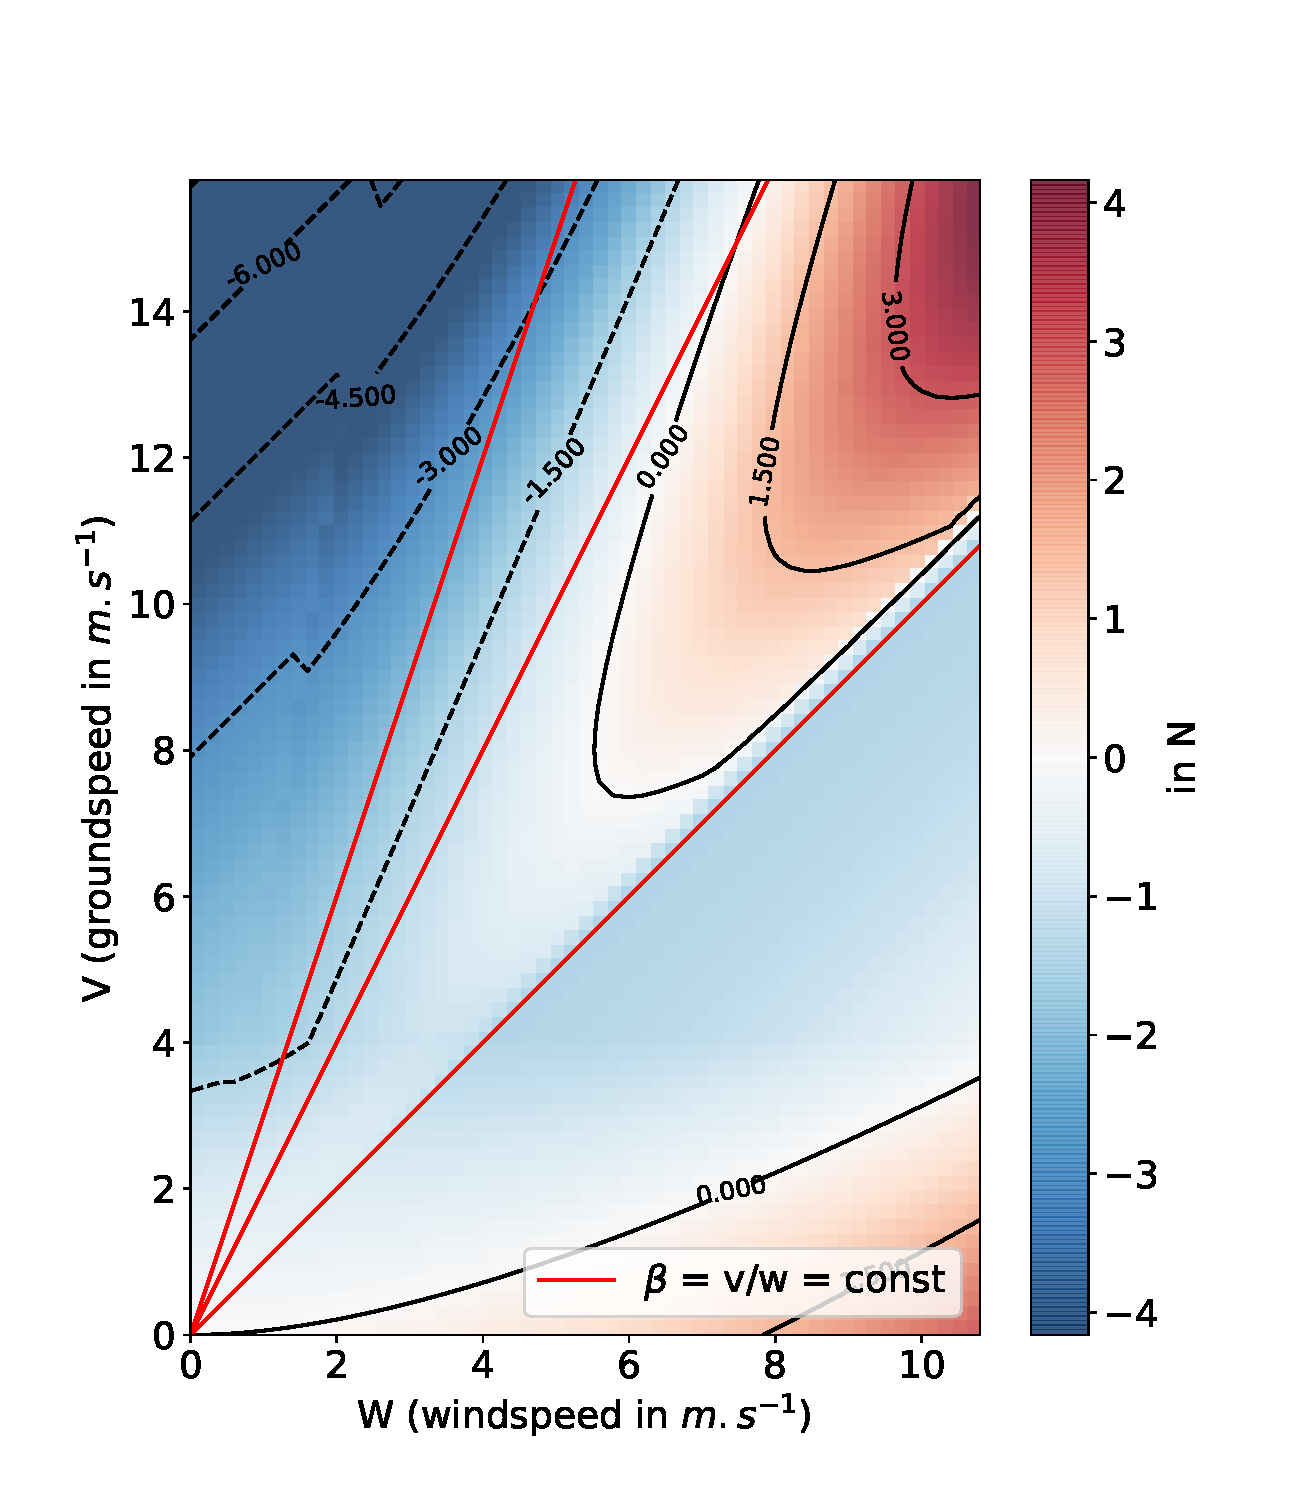
\includegraphics[width = 0.22\textwidth]{images/part6/naca6412-8a-78-10-5-3-470-6__total.pdf}
    
    \caption{Total force (left) and thrust (right) as a function of groundspeed and windspeed. Lines of constant speed ratio shown in red (with $\beta$ = 1, 2 and 3)}

    \label{fig:pythonresults}
\end{figure}

Iterating over various possible inputs then enabled us to converge to a more adequate propeller. From the model, it was found that a higher operating RPM would increase the overall efficiency of the propeller due to the higher operating Reynolds number. The chosen gear ratio to set the RPM operating range resulted from a compromise between propeller efficiency and safety of operations. It was found that using a gear ratio of 1 yielded an operating Reynolds number of about $1\times10^5$ at the mid-span, which was on the lower limit of what was deemed acceptable. This meant that for $40.6 \mathrm{cm}$ wheels and operating at $10 \mathrm{m/s}$, the RPM of the propeller was 463. 

The number of blades was also assessed. Given the diameter limitation of 80cm, the blade count had to be chosen to allow the propeller to generate enough thrust at the specified RPM (defined from manufacturing requirements later). Increasing the number of blades also meant a greater impact on the budget. From the model output, it was determined that a minimum of three blades would output the required amount of thrust while maintaining an efficient blade geometry as shown in Figure \ref{fig:jprop}.

\begin{figure}[!htbp]
    \centering
    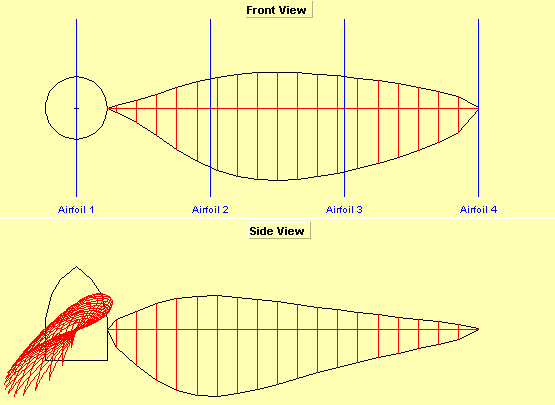
\includegraphics[width= 0.45\linewidth]{images/part6/javaprop2blades.png}
    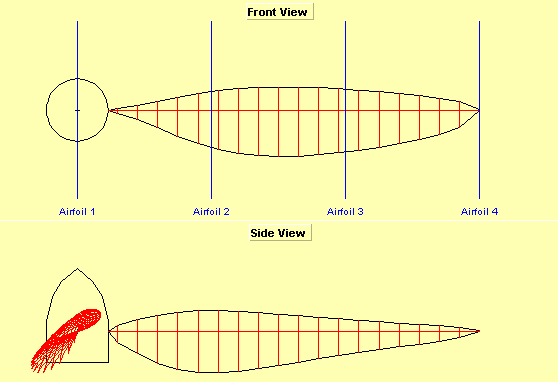
\includegraphics[width= 0.48\linewidth]{images/part6/javaprop3blades.png}
    \caption{JavaProp output geometry for a 2-bladed propeller (left) and a 3-bladed propeller (right) designed for equal thrust output}
    \label{fig:jprop}
\end{figure}

Several blade profiles were tested to assess their impact on the performance of the vehicle. The lift-to-drag ratios of the profiles were compared, as shown on Figure \ref{fig:clcdalpha}. It is clear from this plot that the NACA 6412 had a significantly better performance than the other two. Further investigations were conducted using the theoretical model. The main observation was that a higher cambered aerofoil blade profile would have a broader range of pitch over which the thrust was high in comparison to low camber and symmetrical aerofoil blade profiles. This is illustrated on Figure \ref{fig:aeroprofiles}. The NACA 6412 profile was chosen due to its higher performance at the relevant Reynolds number range as shown on Figure \ref{fig:clcdalpha}.

\begin{figure}[!htbp]
    \centering
    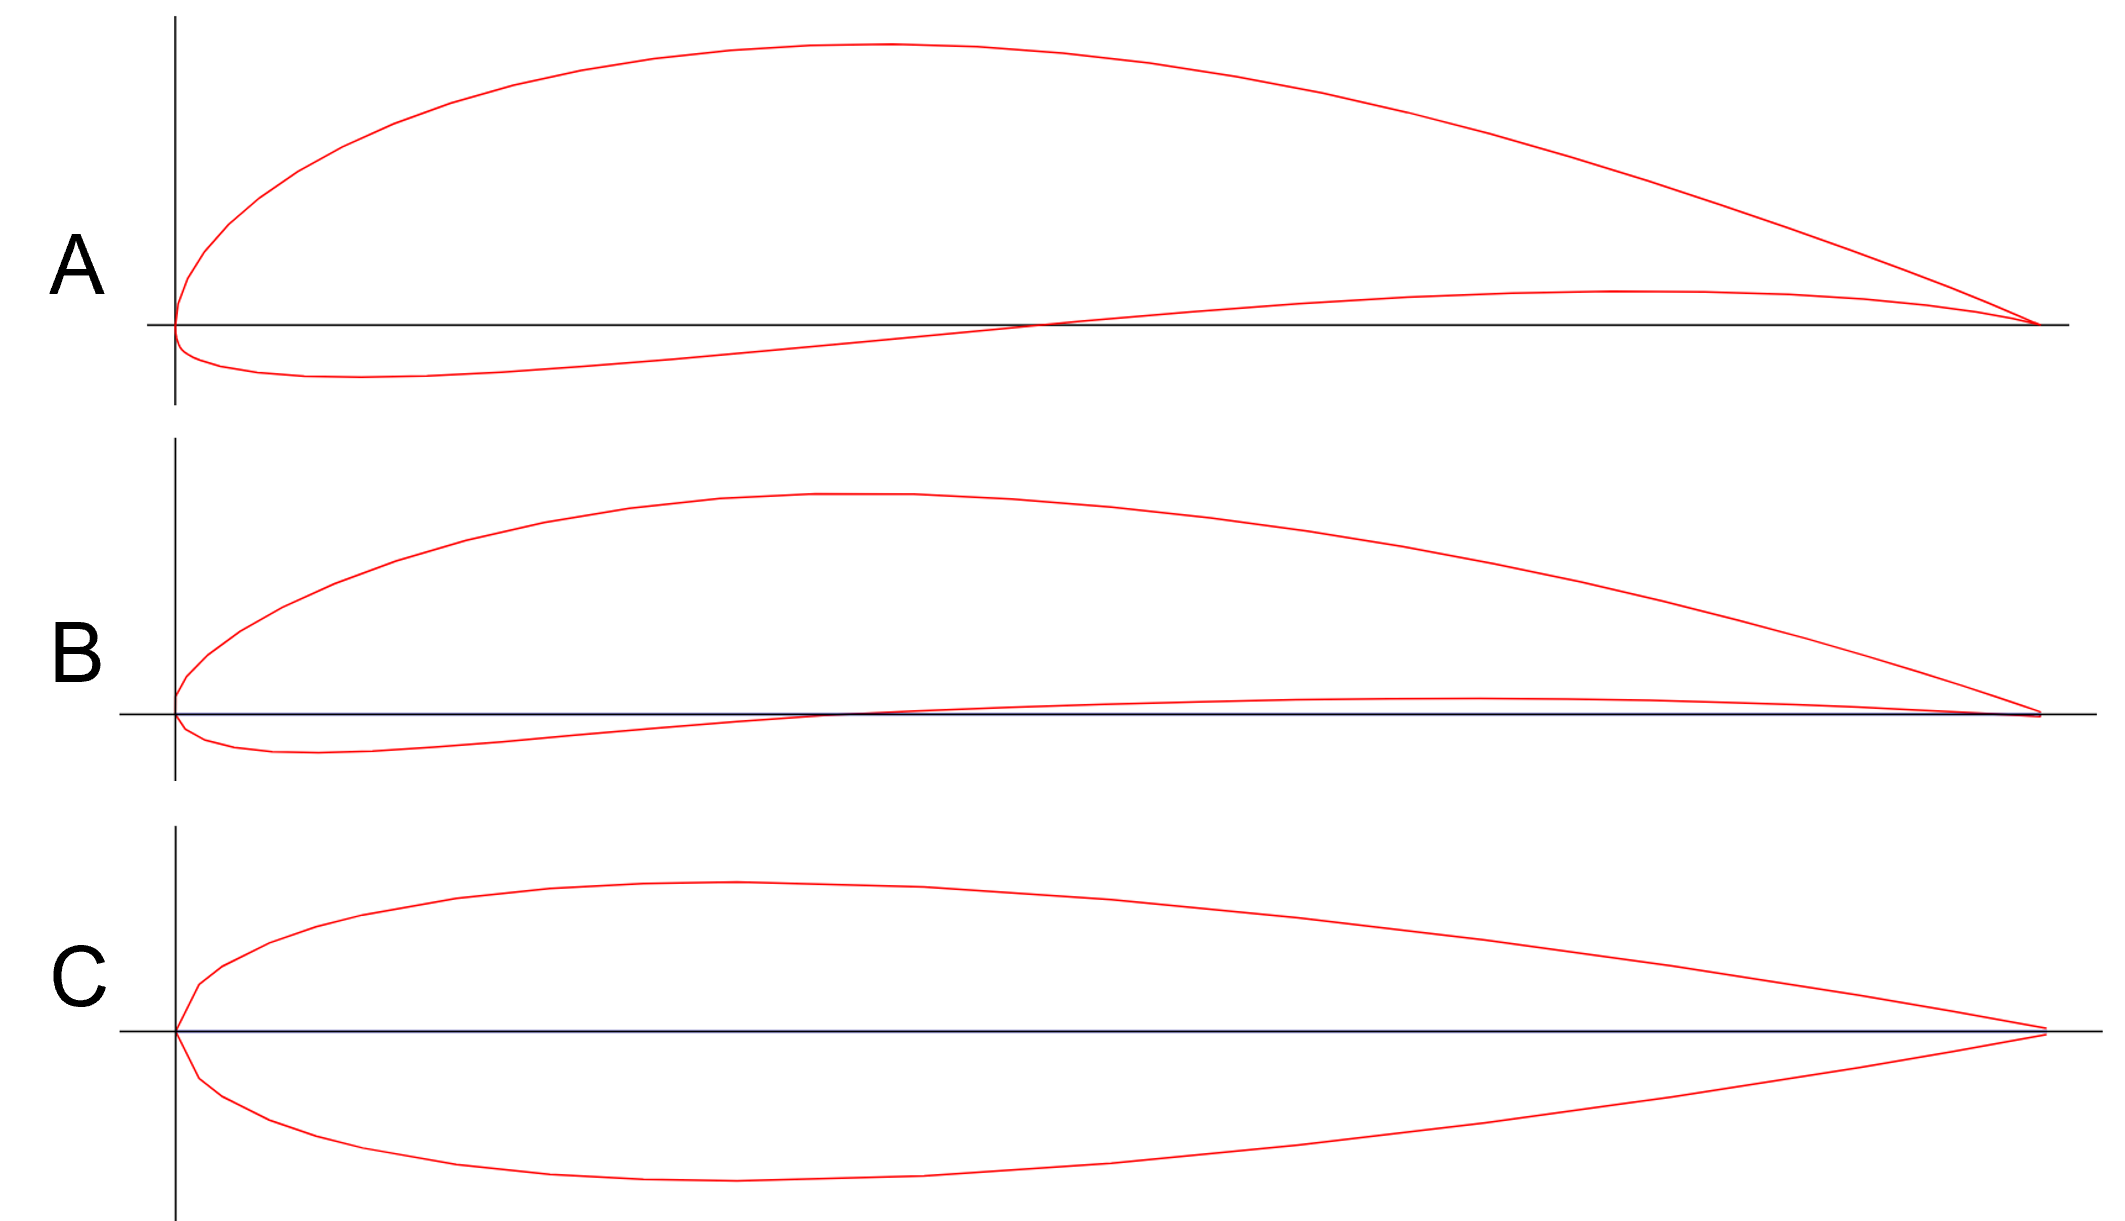
\includegraphics[width=0.4\linewidth]{images/part6/bladeprofiles.png}
    \label{fig:bladeprofiles}
    \caption{Assessed blade profiles: mh112 (A), NACA 6412 (B), NACA 0016 (C)}
\end{figure}

\begin{figure}[!htbp]
    \centering
    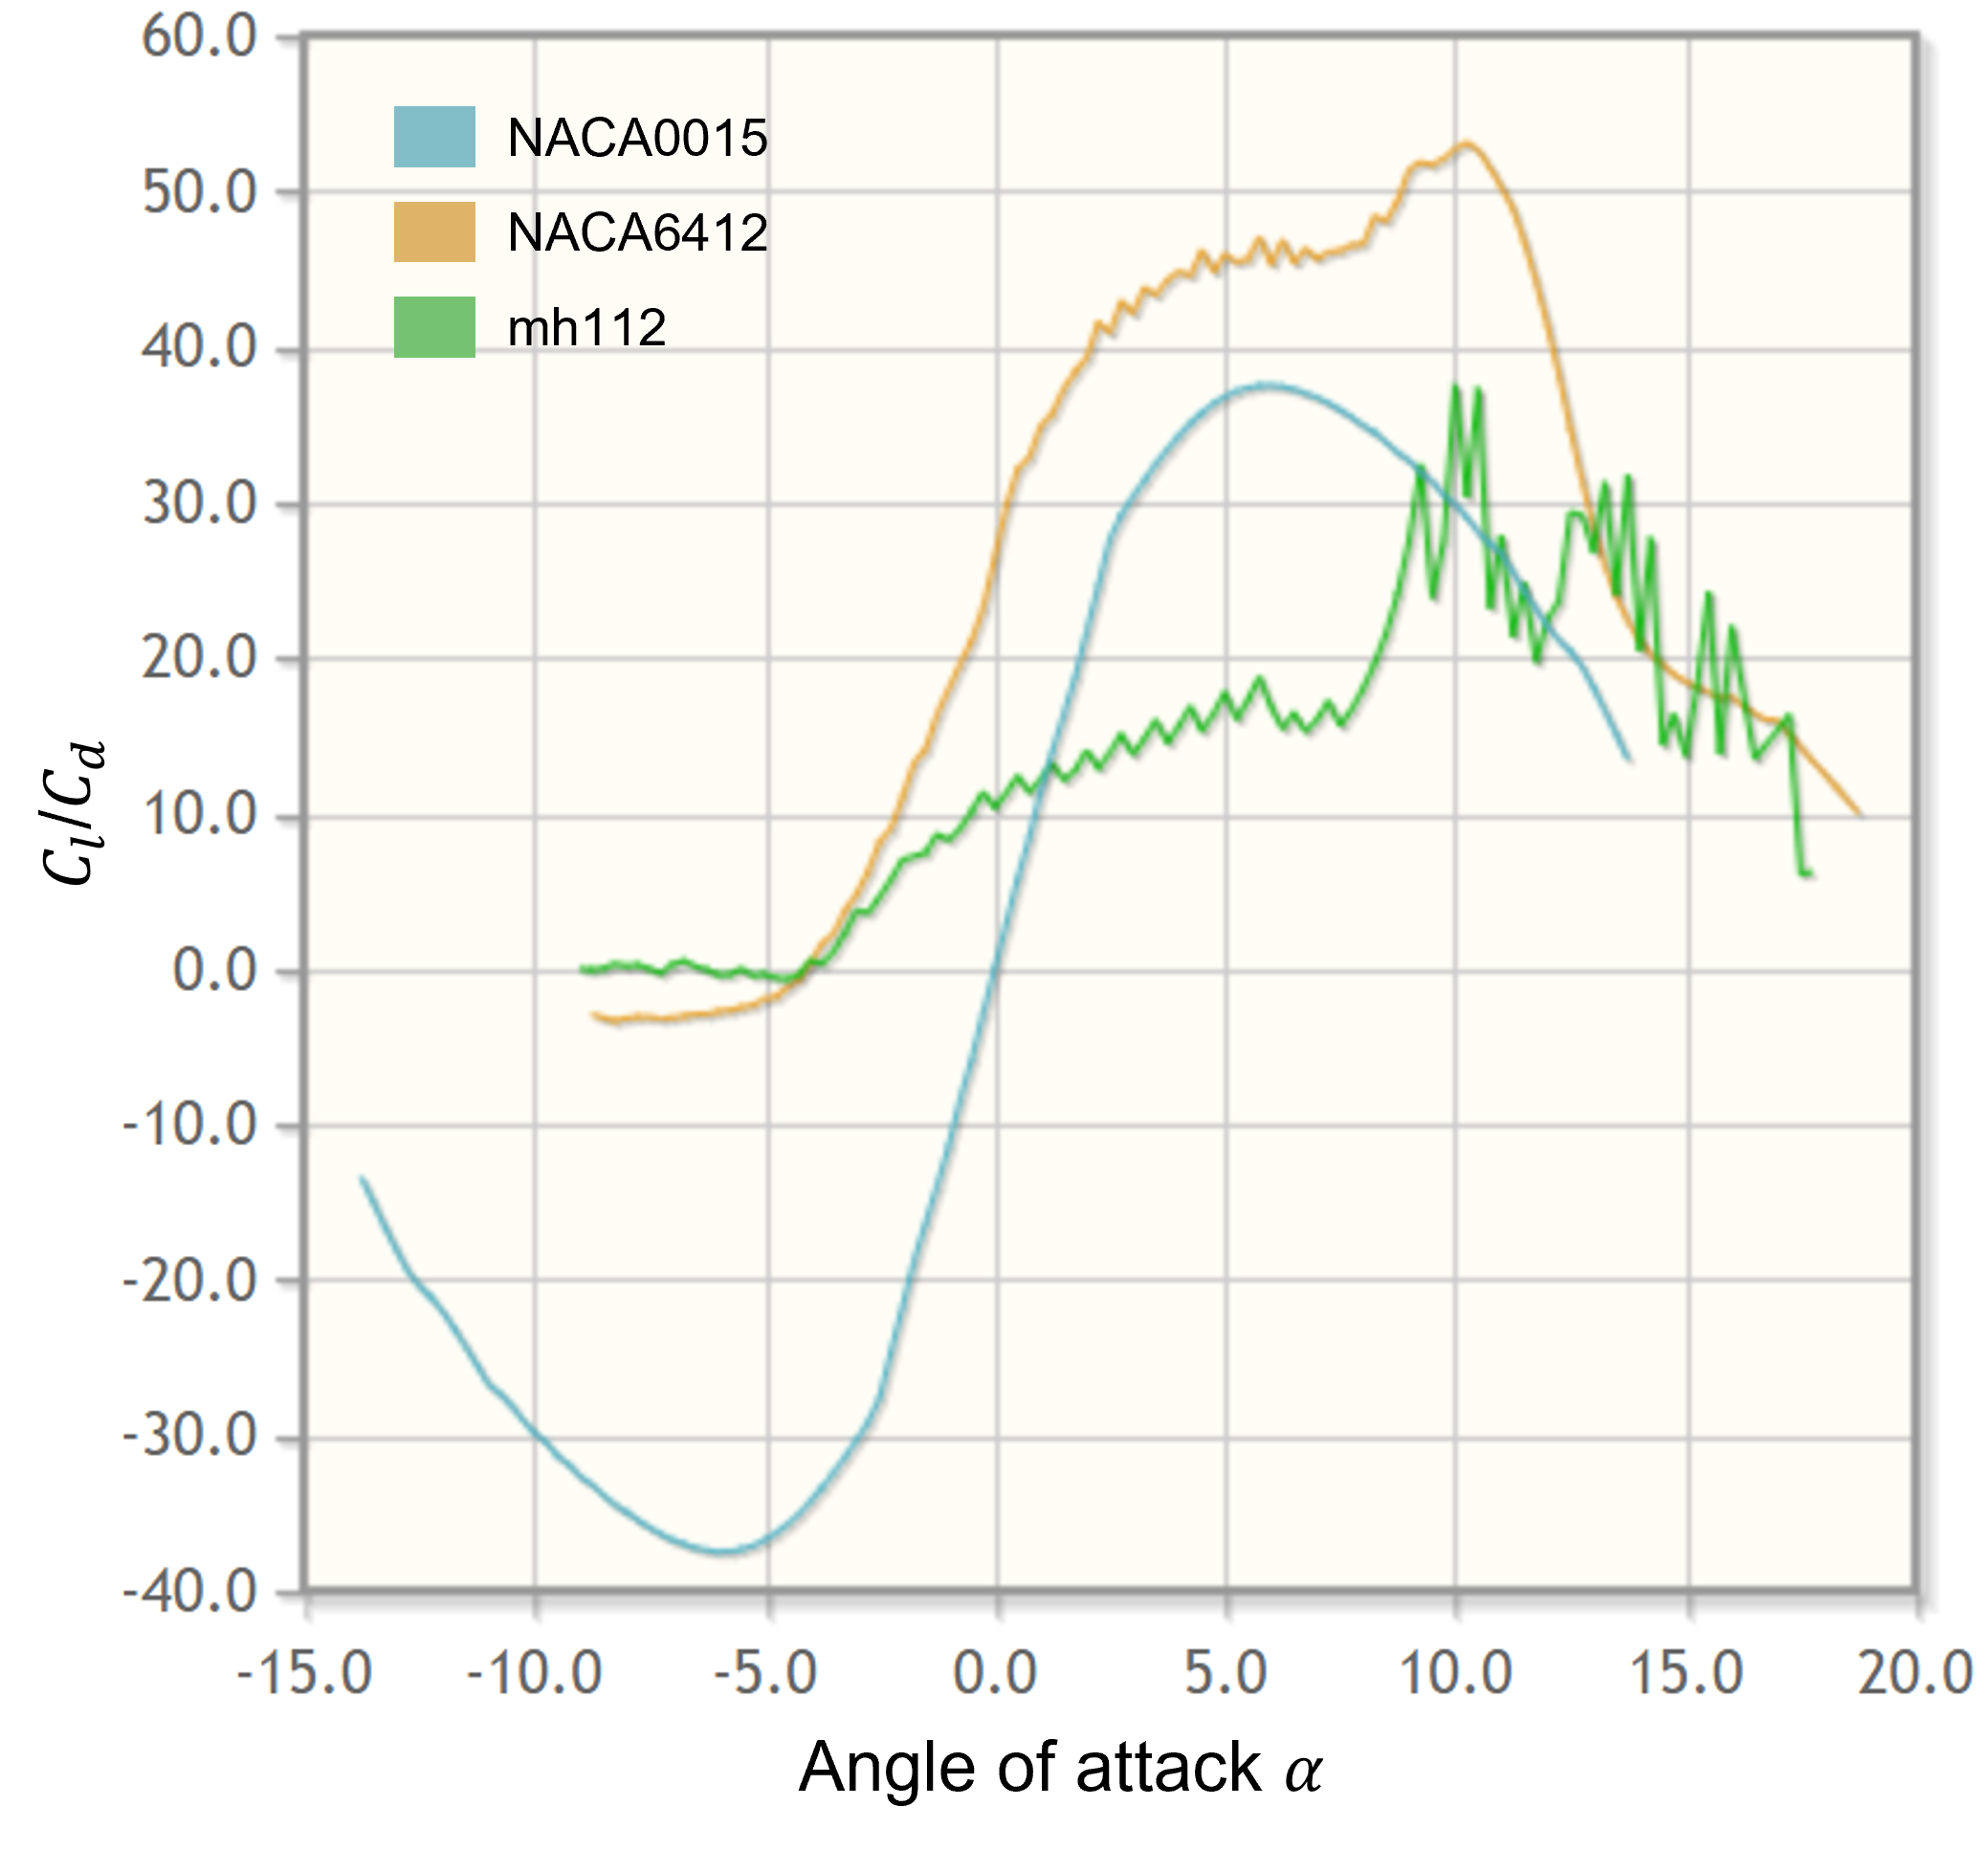
\includegraphics[width = 0.5\linewidth]{images/part6/clcdalpha.png}
    \caption{$C_l/C_d$ as a function of $\alpha$ for different blade profiles ($\mathbf{Re} = 1\times10^{05}$)}
    \label{fig:clcdalpha}
\end{figure}

\begin{figure}[!htbp]
    \centering
    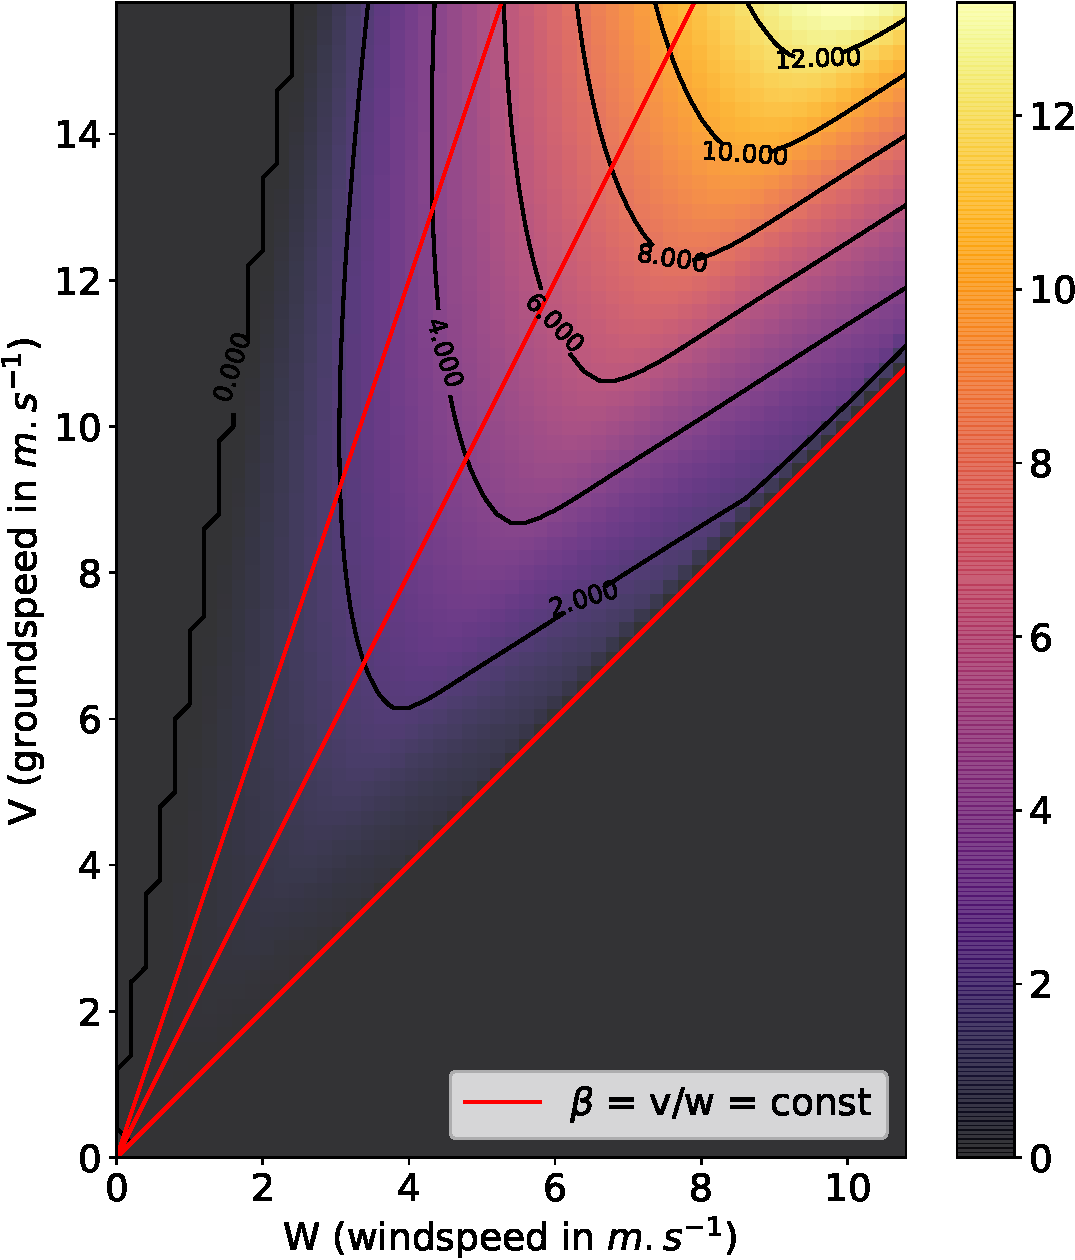
\includegraphics[width =0.1465\textwidth]{images/part6/naca0016.pdf}
    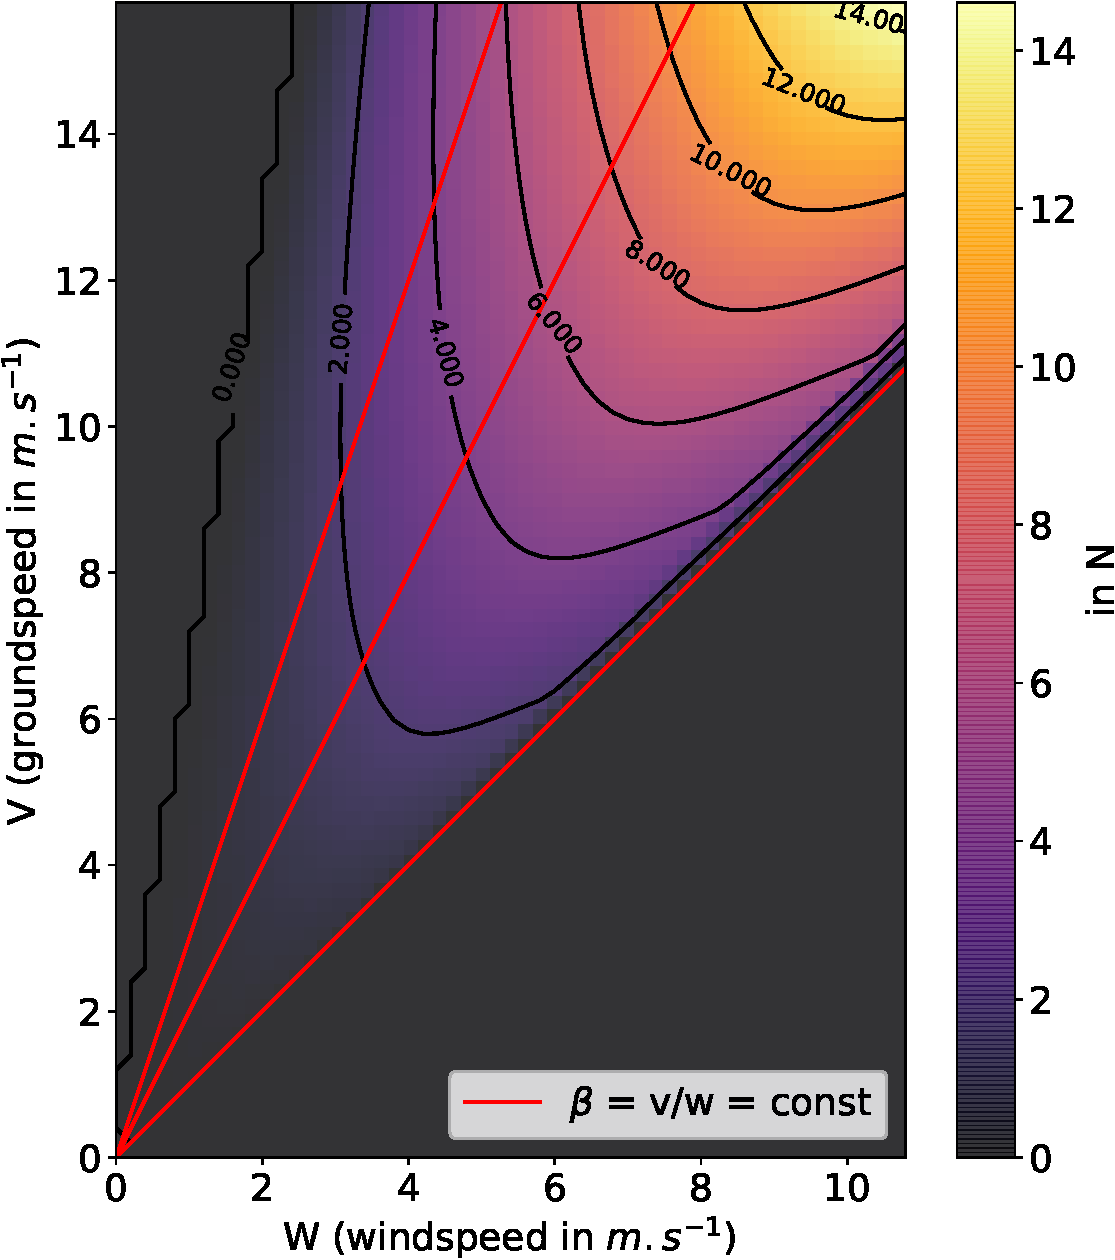
\includegraphics[width =0.152\textwidth]{images/part6/naca6412.pdf}
    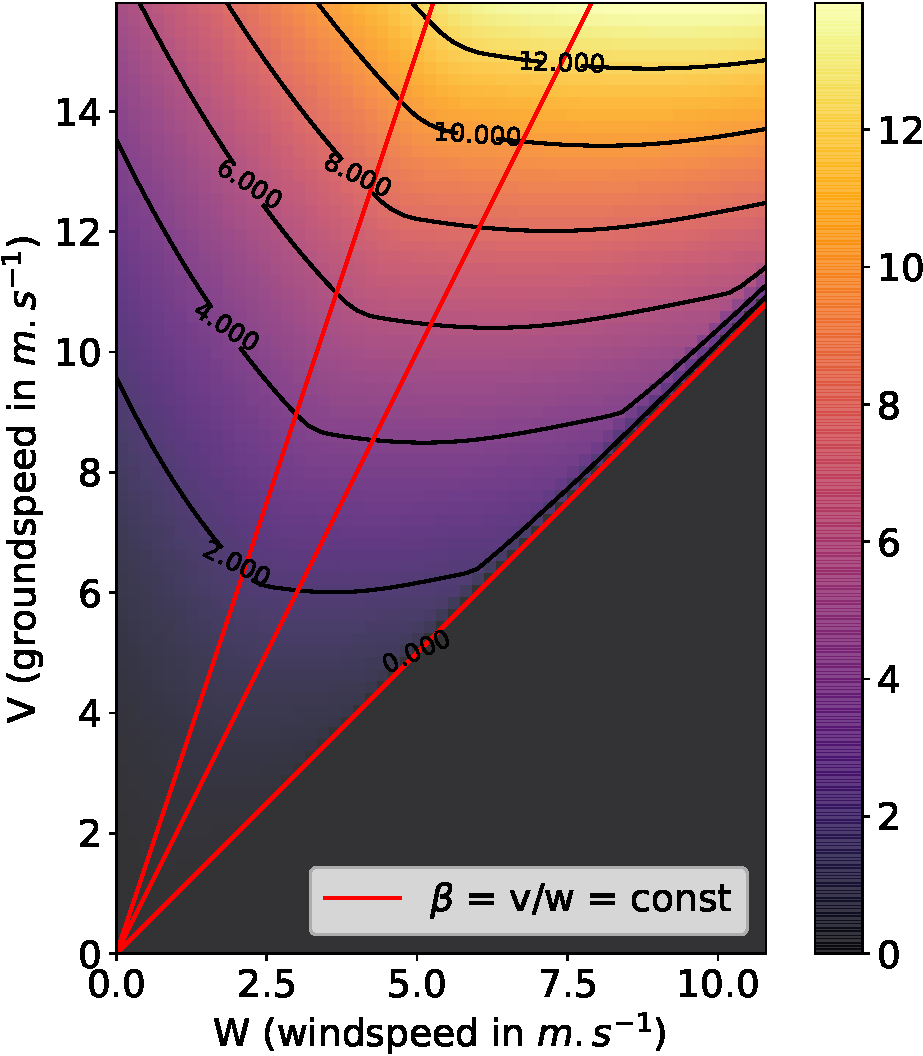
\includegraphics[width =0.15\textwidth]{images/part6/mh112.pdf}
    \caption{Propeller thrust as a function of groundspeed and windspeed. From left to right: NACA 0016, NACA 6412, mh112}

    \label{fig:aeroprofiles}
\end{figure}

It was then possible to converge towards a more efficient propeller design. Due to budgeting, and the limited impact of blade number on efficiency as stated before, the blade number was set to 3.

\subsection{Manufacturing}

The manufacturing process of the propeller had a high impact on the design choices. It was initially decided that the best course of action would be to buy an off-the-shelf propeller and in parallel, further improve a custom geometry and manufacture it further down the line. After surveying the market for off-the-shelf propellers in the size range required, it was made clear that there were not any suitable options for application in this project. The available rotors being designed for model aircraft and other similar applications did not feature an adequate pitch nor the possibility of modulating it. This meant that modifications would have to be made to the blades. Being made for high RPM applications (2000+ RPM) and a lower pitch than desired, restructuring the blades and using them on a custom hub would lead to safety concerns. Also, the lower efficiency provided by propellers featuring a low number of blades (2 in this case) was a non-negligible drawback in this case, where efficiency is key. Consequently, as the price for off-the-shelf propellers was quite high, and the predicted performance quite low, more focus and effort was put on designing and manufacturing the custom propeller.

Several possibilities were outlined when it came to manufacturing the propeller, of which were carbon fibre layup, aluminium machining, metal printing, and PLA 3D printing. Each one of these materials had mechanical properties suitable for high-RPM operations as determined by modelling the blades as rectangular and finding the tensile strength of the root which is highly stressed under centrifugal loading (Table \ref{fig:mattable}).

\begin{table}[!htbp]
    \centering
    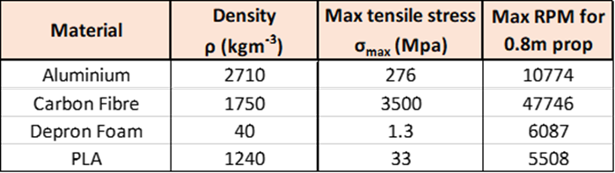
\includegraphics{images/part6/materialstable.png}
    \caption{Material strength analysis for propeller}
    \label{fig:mattable}
\end{table}

Due to the lack of experience in the team required to perform carbon fibre manufacturing and high associated costs, this option was ruled out. A mix of aluminium and PLA 3D printing was chosen as this would exploit the strength of aluminium for load bearing components, and the low cost, easy changeability of PLA parts for the most aerodynamic sections of the blade.

The mid-section of the propeller would be 3D printed in PLA in two parts (Due to the vertical orientation of parts to align the layer lines with the flow direction) whilst the tips and roots of the blades would be 3D printed in aluminium and held together by a rod running through all sections. This meant that the centrifugal load on the PLA sections would be transferred to the aluminium tip, connected to the root by the spar. Doing this ensures the 3D prints experience only compressive loads and cannot delaminate. This combination limits the costs and weight of the blades, with a roughly 68\% mass saving over an entirely aluminium equivalent. An additional benefit was the possibility to reassemble the blades with various midsections to generate improved geometries from testing, whilst retaining the aluminium root and tips. These geometries could then easily be replaced and fitted on the blade rods. An exploded view of this design is shown in Figure \ref{fig:propExploded} and explained in further detail later.

Propeller blades experience maximum stress at their root due to the centripetal force produced by the mass above them. Using a simple rectangular blade model, the minimum diameter of an aluminium spar required to carry the centripetal load at 2000 RPM (significantly higher than operational speeds) and a safety factor of 2  would be 2.1 mm. The decision was therefore made to use a 4 mm diameter spar as this would suitably handle the expected loads whilst comfortably fitting within the thickness of the blade. Integrating a thread into one end for securing nuts would yield a thread stripping shear strength in excess of 350 kg (3.48 kN), whilst the propeller would see loads up to 60 kg (580 N) at 2000 RPM. This result is typical of the safety margins of the propeller design, and even with the imperfect manufacture of components, the likelihood of failure is incredibly low.

An initial design of the custom propeller was achieved before Christmas as shown in Figure \ref{fig:propExploded}. In total, 8 different parts were designed. Some of these were to be manufactured by EDMC (4, 5, and 7). The PLA 3D-printed parts were to be manufactured directly by the team (1-3). Due to technical issues with the metal 3D printer, the initially designed roots and tips (4 and 5) had to be replaced with suitable alternatives, so the roots were then also 3D printed in PLA (4*), while the tips were replaced with water-jet cut aluminium sheets (5*). The new tip replacement parts were then welded to the spar, as initially planned, such that the load experienced by the tips was transferred to the spar. These changes are shown in Figure \ref{fig:propExploded} by the initial and revised design following these manufacturing complications, with parts outlined in Table \ref{tab:propParts}.

\begin{figure}[!htbp]
    \centering
    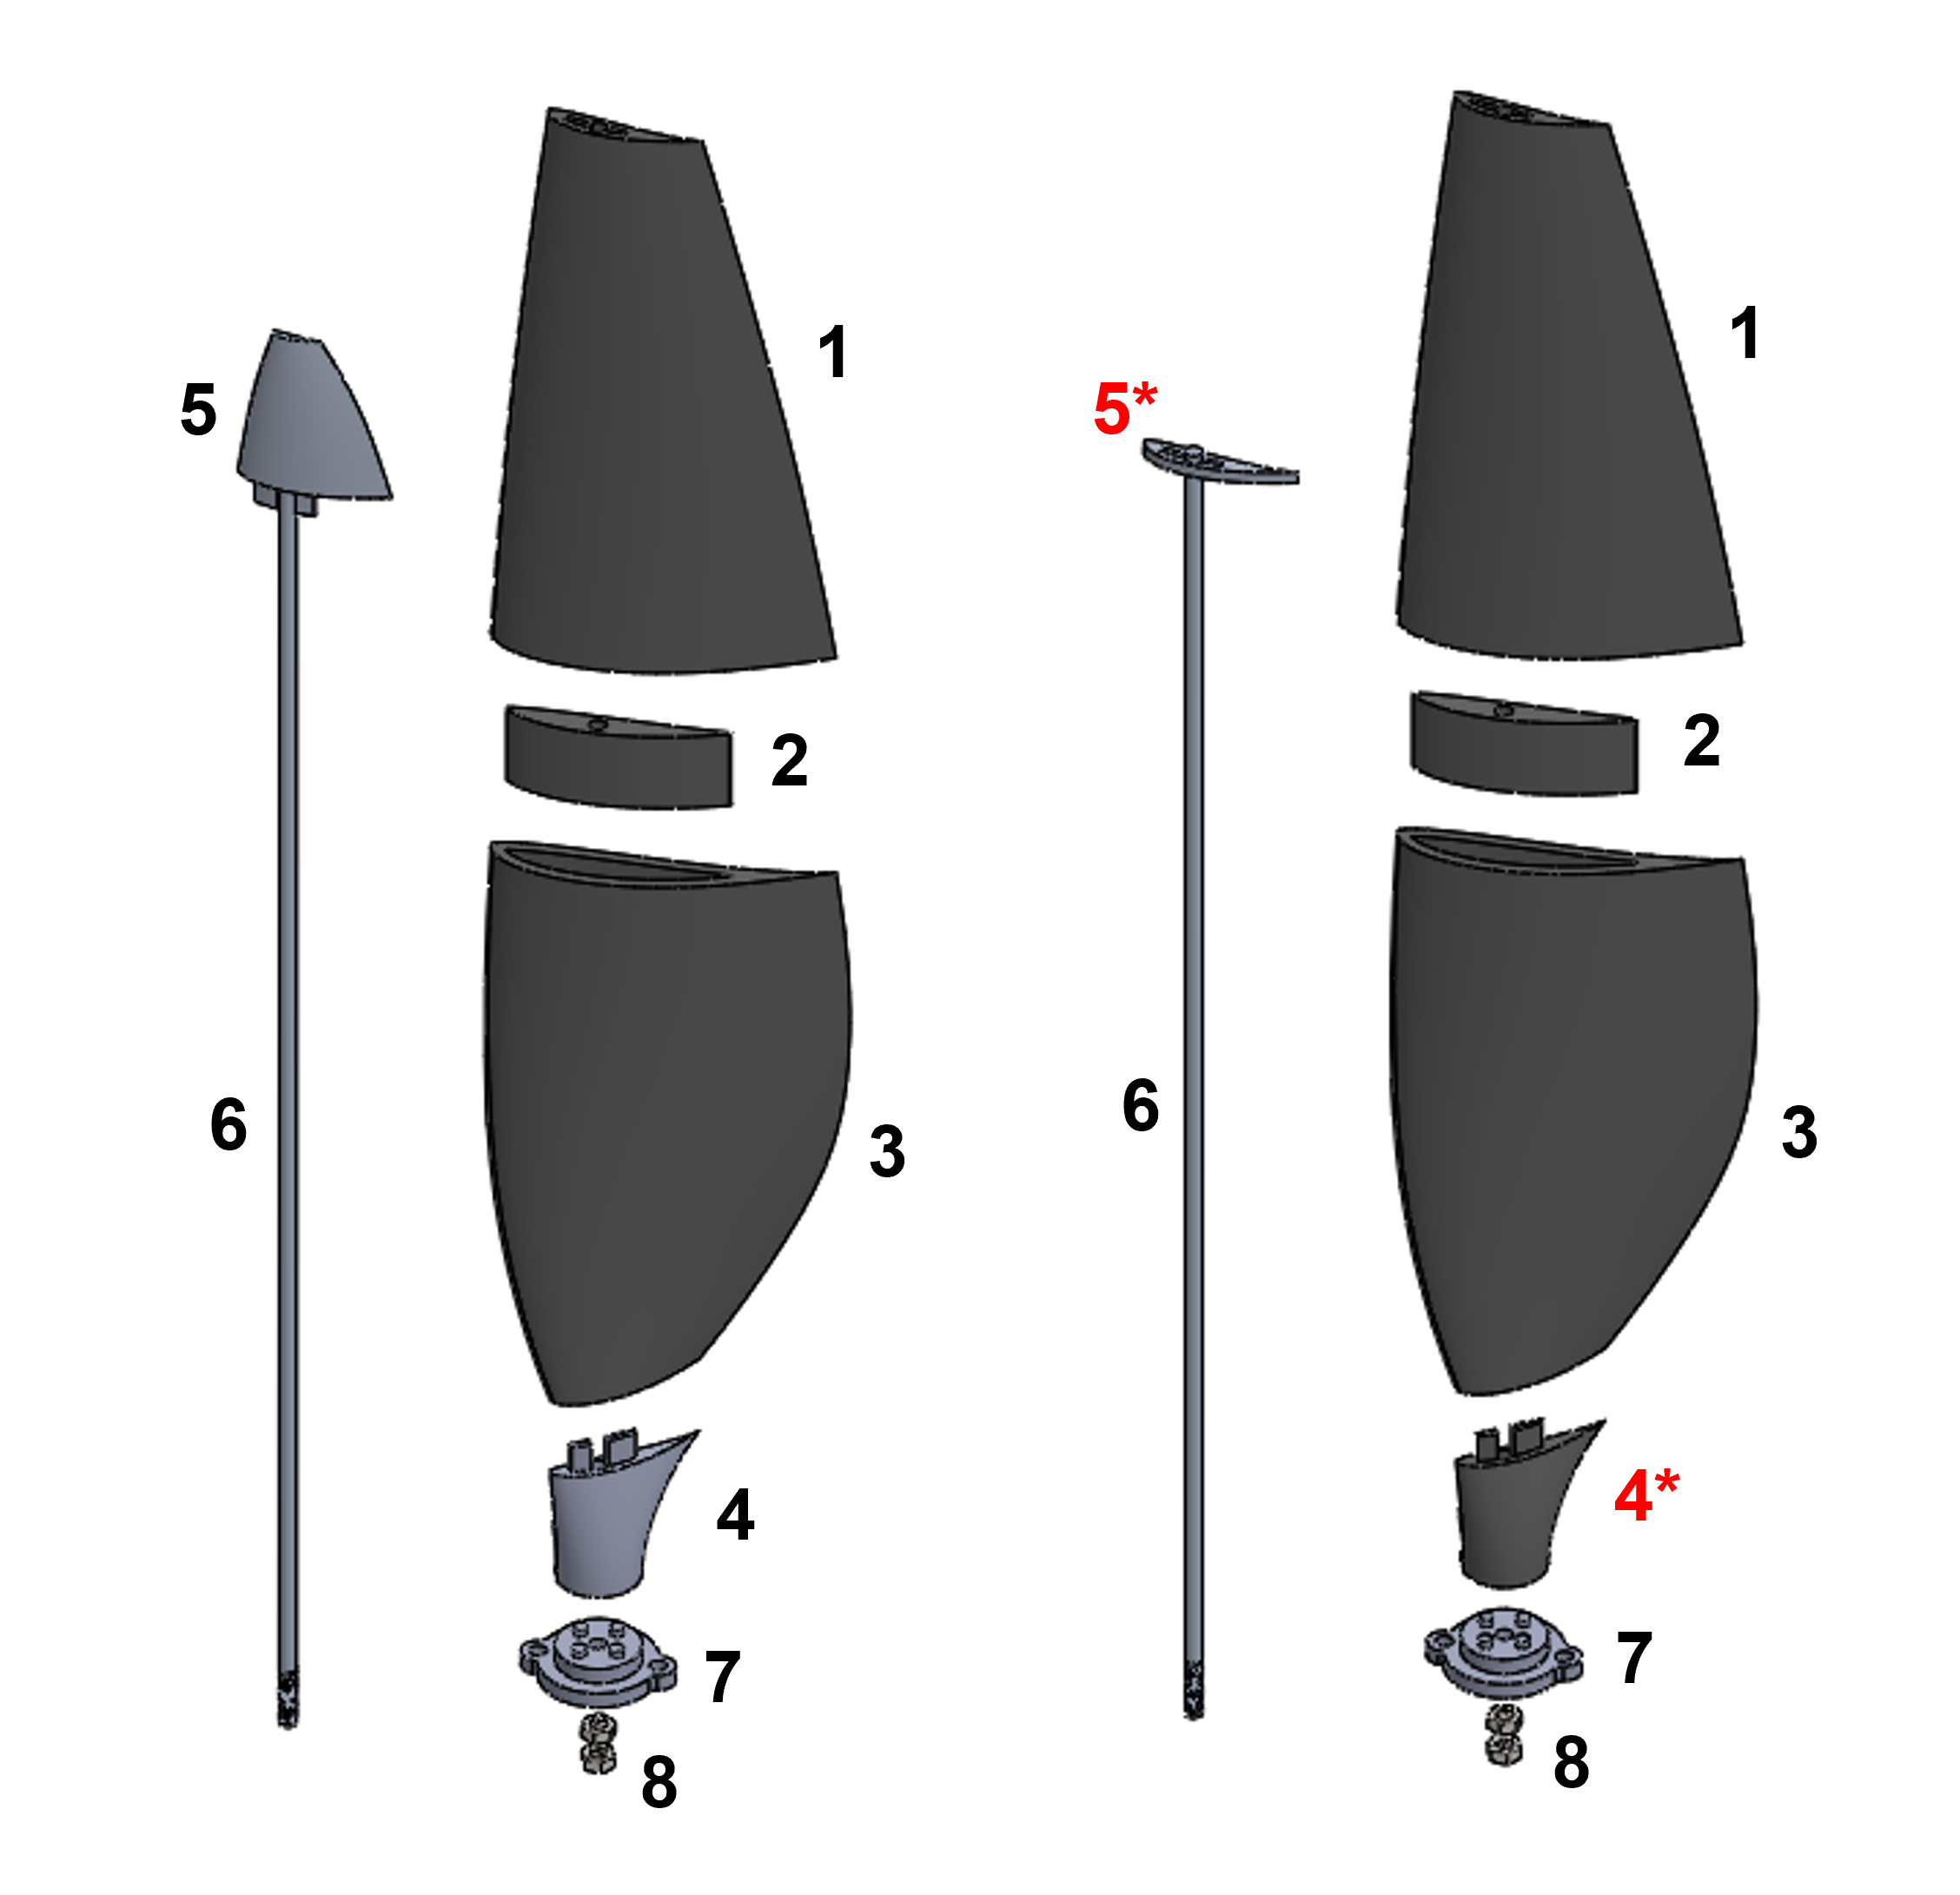
\includegraphics[width=0.7\linewidth]{images/part6/propExploded.png}
    \caption{Exploded view of final propeller design (left) and revised design (right)}
\label{fig:propExploded}
\end{figure}

\begin{table}[h]
\centering
\begin{tabular}{cllc}
\rowcolor[HTML]{C0C0C0} 
\multicolumn{1}{l}{\cellcolor[HTML]{C0C0C0}\textbf{Part No.}} & \textbf{Description}         & \textbf{Material} & \multicolumn{1}{l}{\cellcolor[HTML]{C0C0C0}\textbf{Quantity}} \\
1                                                             & 3D printed upper section     & PLA               & 1                                                             \\
2                                                             & 3D printed alignment coupler & PLA               & 1                                                             \\
3                                                             & 3D printed lower section     & PLA               & 1                                                             \\
4                                                             & Metal 3D printed root        & Aluminium         & 1                                                             \\
4*                                                            & 3D printed root              & PLA               & 1                                                             \\
5                                                             & Metal 3D printed tip         & Aluminium         & 1                                                             \\
5*                                                            & Water-jet cut tip            & Aluminium         & 1                                                             \\
6                                                             & Ø4mm propeller spar          & Aluminium         & 1                                                             \\
7                                                             & CNC machined root mount      & Aluminium         & 1                                                             \\
8                                                             & Securing nuts                & Stainless Steel   & 2                                                            
\end{tabular}
\caption{Propeller blade table of parts}
\label{tab:propParts}
\end{table}

After much 3d print testing to ensure suitable mass, strength, tolerances, and surface finish, two sets of final blades were produced with a layer height of 0.1 mm and infill of 20\%. The surface was then smoothed with 140 to 3000 grit sandpaper to remove all traces of layer lines that could interfere with the flow and finished with brass polish. Due to minor unavoidable warping with the prints, small gaps existed between the assembled parts, so were filled with excess PLA scraps and glued together. Each blade was then fully assembled with the additional aluminium components and nuts secured with thread locking adhesive to prevent vibration loosening during tests. Figure \ref{fig:bladeComplete} displays the completed blade ready for insertion in the hub.

\begin{figure}[!htbp]
    \centering
    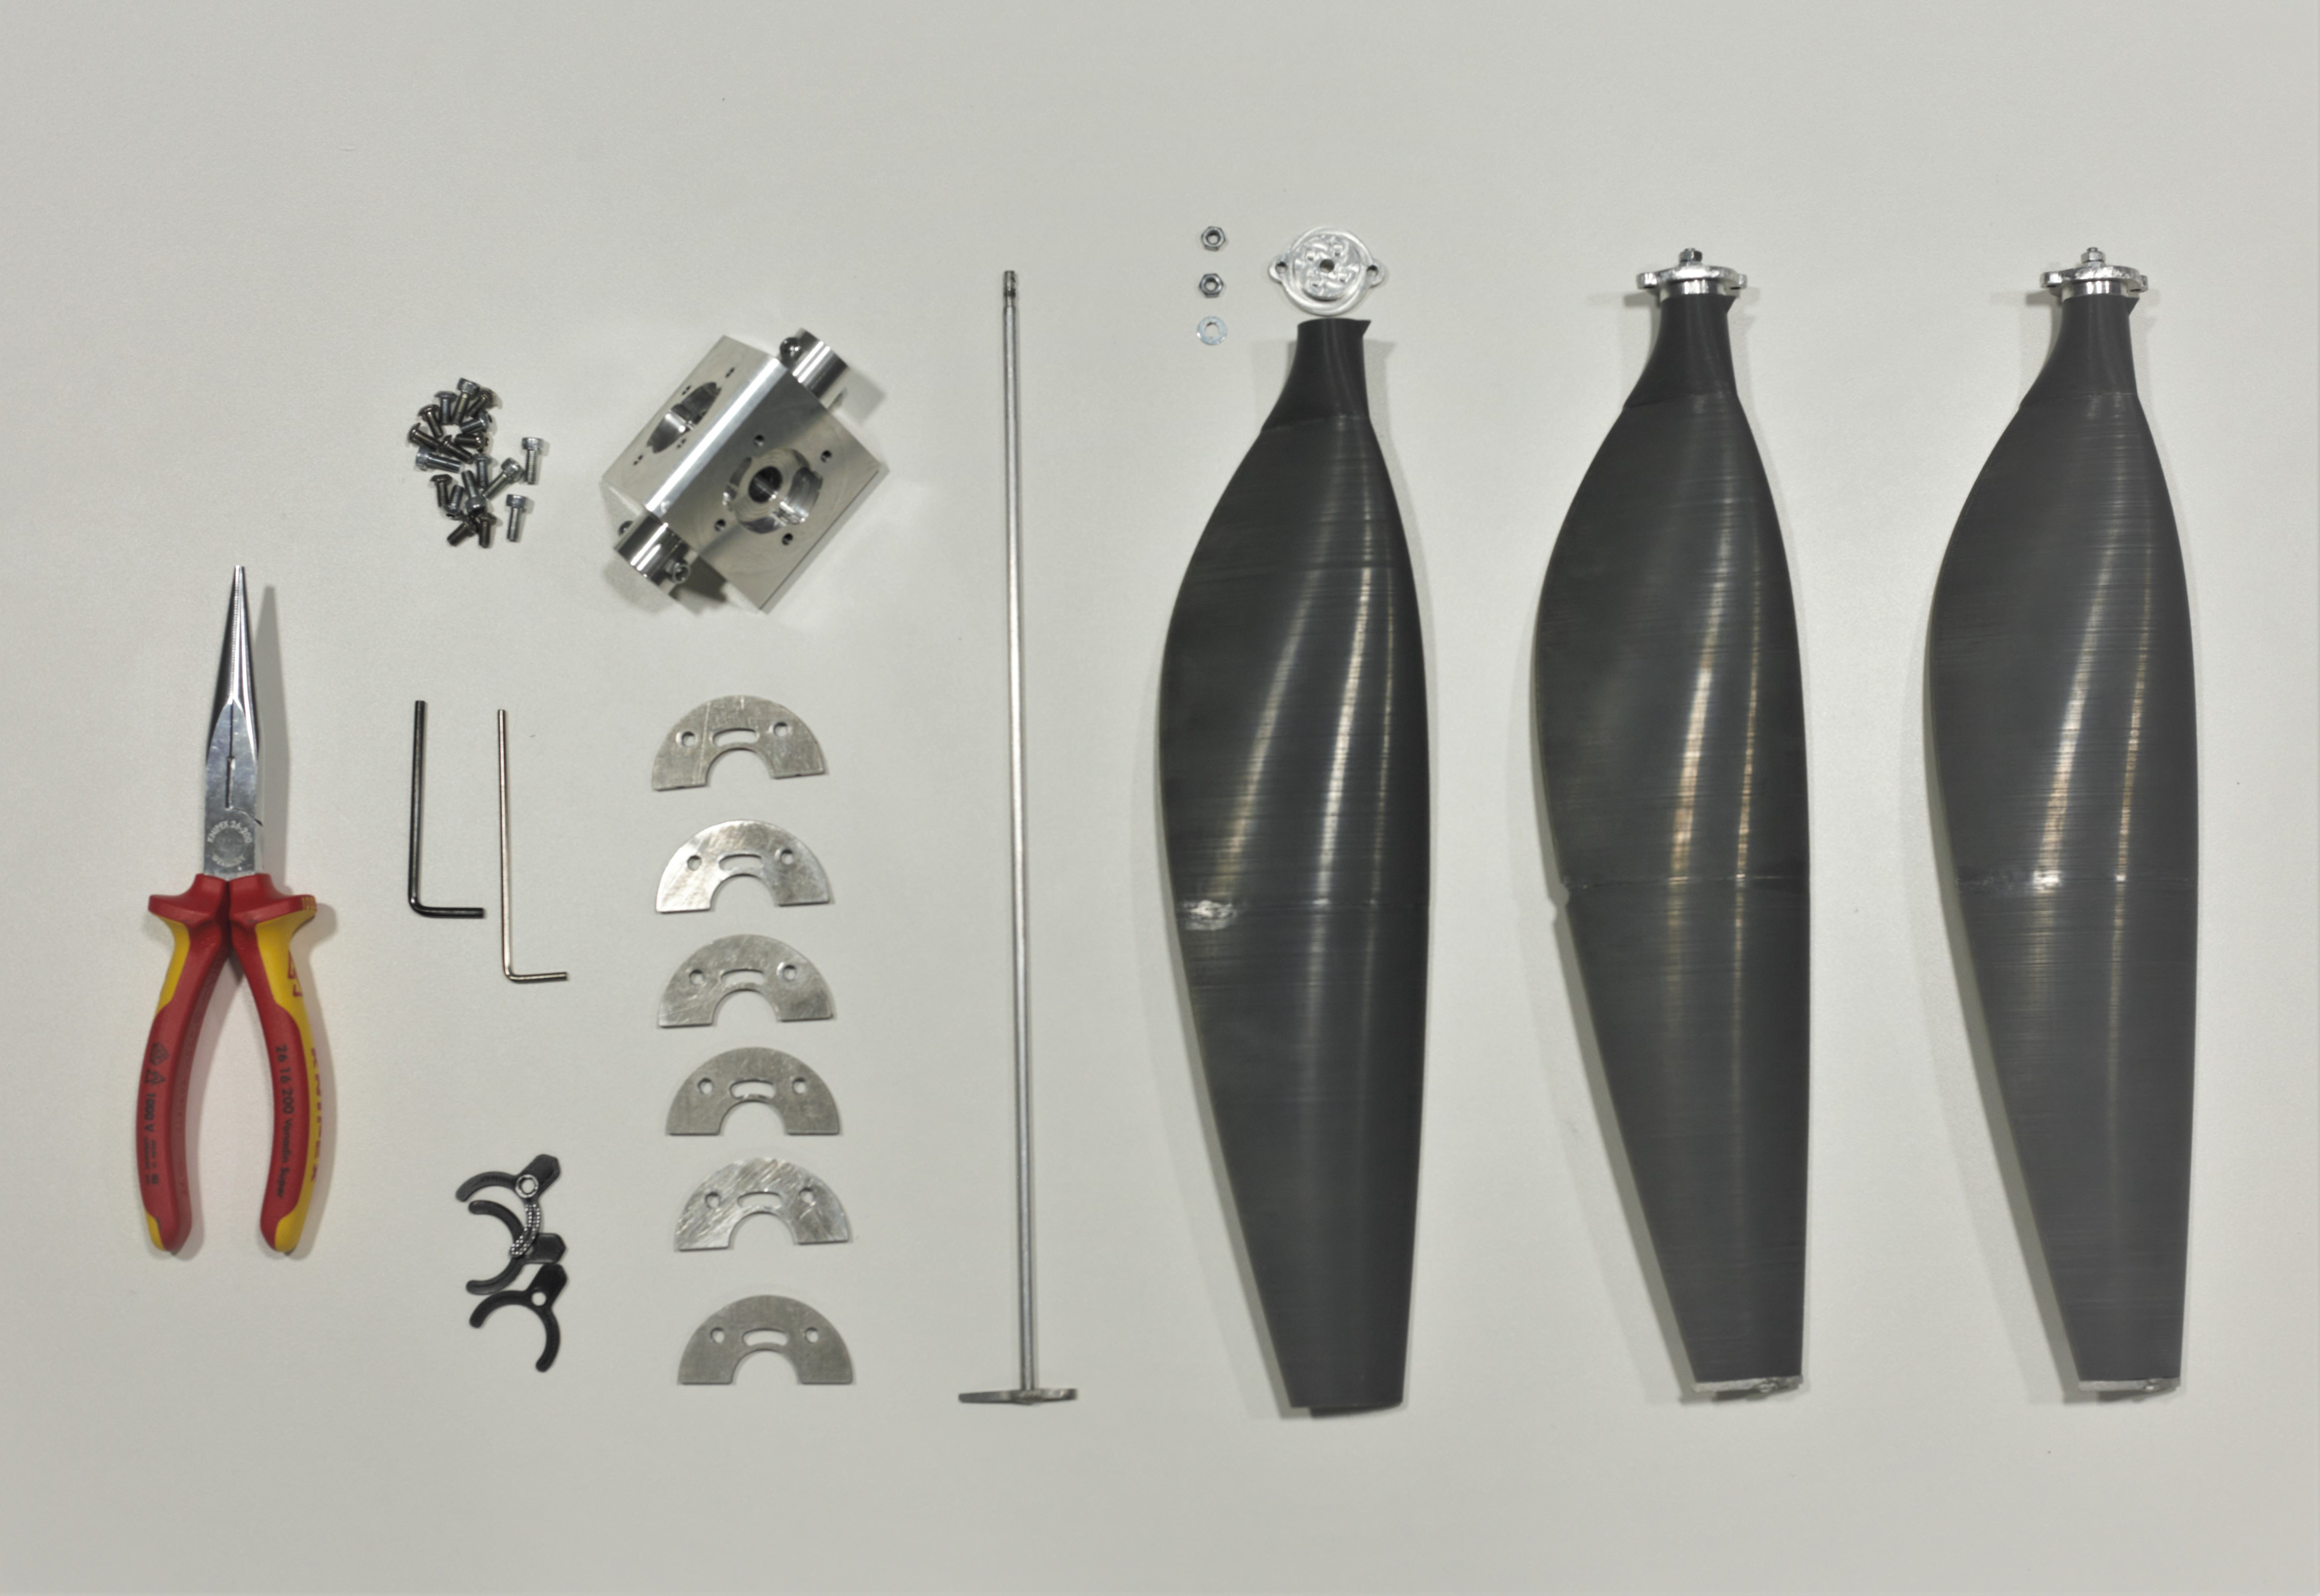
\includegraphics[width=0.7\linewidth, angle=180]{images/part6/buggabugga.jpg}
    \caption{Final manufactured propeller disassembled and all the tools required to assemble it.}
\label{fig:bladeComplete}
\end{figure}

